% diagrams-Bd.tex
\begin{hcarentry}[updated]{diagrams}
\report{Brent Yorgey}%05/15
\status{active development}
\participants{Daniel Bergey, Jan Bracker, Christopher Chalmers, Daniil Frumin,
  Allan Gardner, Andrew Gill, 
  Niklas Haas, John Lato, Chris Mears, Jeff Rosenbluth, Michael Sloan, Ryan Yates, Brent Yorgey}
\makeheader

The diagrams framework provides an embedded domain-specific language
for declarative drawing.  The overall vision is for diagrams to become
a viable alternative to DSLs like MetaPost or Asymptote, but with the
advantages of being \emph{declarative}---describing what to draw, not
how to draw it---and \emph{embedded}---putting the entire power of
Haskell (and Hackage) at the service of diagram creation.  There is
still much more to be done, but diagrams is already quite
fully-featured, with a comprehensive user manual, a large collection
of primitive shapes and attributes, many different modes of
composition, paths, cubic splines, images, text, arbitrary monoidal
annotations, named subdiagrams, and more.

%**<img width=400 src="./arrows.jpg">
%*ignore
\begin{center}
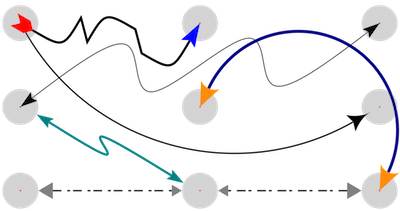
\includegraphics[width=0.47\textwidth]{html/arrows.jpg}
\end{center}
%*endignore

\subsubsection*{What's new}

Since the last HCAR edition, diagrams 1.3 was released in April.
New features include:
\begin{compactitem}
\item Computing intersection points between paths
\item Support for generalized affine maps between different vector
  spaces, including projections
\item New backends: \texttt{diagrams-html5} generates Javascript to draw on an
  HTML canvas; \texttt{diagrams-pgf} generates PGF code suitable for
  inclusion in a \TeX document
\item Better interface for recompilation looping via the command line
\item Generalized numerics: diagrams are now parameterized by a
  suitable numeric type, rather than having \texttt{Double} baked in
\item A refactoring to use the \texttt{linear} package instead of
  \texttt{vector-space}
\end{compactitem}


%**<img width=350 src="./kaleidoscope.jpg">
%*ignore
\begin{center}
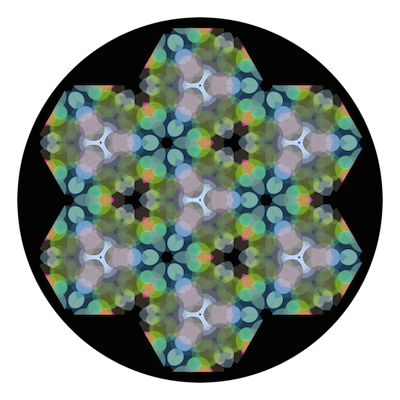
\includegraphics[width=0.45\textwidth]{html/kaleidoscope.jpg}
\end{center}
%*endignore

\subsubsection*{GSoC}

This coming summer, Ajay Ramanathan will work under the guidance of
Chris Chalmers to develop a library/API for working with a layered
``Grammar of Graphics'', using \texttt{diagrams} as a foundation.

\subsubsection*{Contributing}

There is plenty of exciting work to be done; new contributors are
welcome!  Diagrams has developed an encouraging, responsive, and fun
developer community, and makes for a great opportunity to learn and
hack on some ``real-world'' Haskell code.  Because of its size,
generality, and enthusiastic embrace of advanced type system features,
diagrams can be intimidating to would-be users and contributors;
however, we are actively working on new documentation and resources to
help combat this.  For more information on ways to contribute and how
to get started, see the Contributing page on the diagrams wiki:
\url{http://haskell.org/haskellwiki/Diagrams/Contributing}, or come
hang out in the \texttt{\#diagrams} IRC channel on freenode.

%**<img width=400 src="./topoform.jpg">
%*ignore
\begin{center}
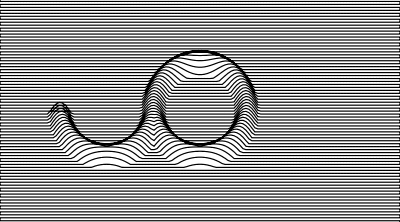
\includegraphics[width=0.4\textwidth]{html/topoform.jpg}
\end{center}
%*endignore

\FurtherReading
\begin{compactitem}
\item \url{http://projects.haskell.org/diagrams}
\item \url{http://projects.haskell.org/diagrams/gallery.html}
\item \url{http://haskell.org/haskellwiki/Diagrams}
\item \url{http://github.com/diagrams}
\item \url{http://www.cis.upenn.edu/~byorgey/pub/monoid-pearl.pdf}
\item \url{http://www.youtube.com/watch?v=X-8NCkD2vOw}
\end{compactitem}
\end{hcarentry}
